\documentclass[10pt,twocolumn,letterpaper]{article}

\usepackage{cvpr}
\usepackage{times}
\usepackage{epsfig}
\usepackage{graphicx}
\usepackage{amsmath}
\usepackage{amssymb}
\usepackage{epstopdf} %% EPS to PDF
\usepackage{multirow}
%\usepackage{subfigure}
\usepackage{subcaption}


%\usepgfplotslibrary{groupplots}
%\pgfplotsset{compat=newest} 
%\pgfplotsset{plot coordinates/math parser=false}

%\usepackage{tikz}
%\usepackage{pgfplots}

%\DeclareGraphicsExtensions{.png,.tex}
%\graphicspath{{figs/}}

%\pgfplotsset{compat=}

% Include other packages here, before hyperref.

% If you comment hyperref and then uncomment it, you should delete
% egpaper.aux before re-running latex.  (Or just hit 'q' on the first latex
% run, let it finish, and you should be clear).
\usepackage[breaklinks=true,bookmarks=false]{hyperref}

\cvprfinalcopy % *** Uncomment this line for the final submission

\def\cvprPaperID{****} % *** Enter the CVPR Paper ID here
\def\httilde{\mbox{\tt\raisebox{-.5ex}{\symbol{126}}}}

% Pages are numbered in submission mode, and unnumbered in camera-ready
%\ifcvprfinal\pagestyle{empty}\fi
\setcounter{page}{1}
\begin{document}

%%%%%%%%% TITLE
\title{Tiny ImageNet Challenge}

\author{Jose Krause Perin\\
Stanford University\\
{\tt\small jkperin@stanford.edu}
% For a paper whose authors are all at the same institution,
% omit the following lines up until the closing ``}''.
% Additional authors and addresses can be added with ``\and'',
% just like the second author.
% To save space, use either the email address or home page, not both
}

\maketitle
%\thispagestyle{empty}

%%%%%%%%% ABSTRACT
\begin{abstract}
This report presents results of convolutional neural network architectures based on classic network architectures such as VGG16, VGG19, and ResNet50 applied to the Tiny ImageNet Challenge. The convolutional layers of the proposed networks were loaded from pre-trained models trained in the larger ImageNet challenge, while the fully connected layers were trained from scratch. Subsequently, all layers were fine tuned. All training stages employed data augmentation. The highest classification accuracy of $53.2\%$ was achieved using the ensemble of the modified VGG16, VGG19, and ResNet50 networks.
\end{abstract}

%%%%%%%%% BODY TEXT
\section{Introduction}
% Introduction: this section introduces your problem, and the overall plan for approaching your problem

The Tiny ImageNet challenge has similar format to the ImageNet Large Scale Visual Recognition Challenge (ILSVRC) \cite{ILSVRC15}, which is a well-known image classification and localization benchmark for large scale datasets. As the name suggests, however, the Tiny ImageNet Challenge has a much smaller data set and the images are also smaller. There are a total of 200 classes. Each class has 500 $64\times 64$ training images, resulting in a total of 100,000 images. The validation and testing data sets have a total of 50 images per class, resulting in a total of 10,000 $64\times 64$ images for each data set. 

The ultimate goal in this challenge is to design a convolutional network architecture that achieves the highest classification accuracy possible on the test data set.

My strategy was to modified existing architectures based of VGG16, VGG19, and ResNet50 to be compatible with the smaller images from the Tiny ImageNet data set. I used transfer learning to train the convolutional layers of these networks based on pre-trained models available on \cite{Pretrained-Models}, whereas the fully connected layers were trained from scratch. These pre-trained models were trained on the larger ImageNet challenge. Given the different images sizes, the features may not be perfectly compatible with the Tiny ImageNet figures. Hence, a subsequent fine tuning training stage was realized to update all layers. In all training stages data augmentation was employed in order to mitigate overfitting.

The remainder of this report is organized as follows. Section~\ref{sec:preprocess} briefly describes the preprocessing realized in the training, validation, and testing data sets. Section~\ref{sec:architecture} describes the network architectures proposed and evaluated in this project. Section~\ref{sec:train} describes the strategy adopted to train the networks. Section~\ref{sec:results} presents the results and discussion. Section~\ref{sec:conclusion} concludes the report.

\section{Data preprocessing} \label{sec:preprocess}
% Describe the methods you intend to apply to solve the given problem

The data and evaluation metric for this problem are already well defined. The data was provided on the class website, and the ultimate goal is to design a network architecture that achieves the highest accuracy on the test data set. 

Before we can start training the neural network, the training, validation, and testing data sets must be loaded from JPEG files and preprocessed. This pre-processing has the goal of making the input vectors zero mean and confined between $[-1, 1]$, as the back-propagation algorithm works better under such conditions. The mean image was calculated by averaging all images from the training set. 

In addition to removing the mean and normalizing the data, all images were cropped by 4 pixels in each side, which resulted in the final images used for training, validation, and testing having size $56 \times 56$. 

\section{Network architectures} \label{sec:architecture}

\begin{table*}[t]
	\caption{Proposed network architectures}
	\label{tab:network}
	\centering
	\begin{tabular}{c|c|c}
		\hline
		\textbf{Modified VGG16} & \textbf{Modified VGG19} & \textbf{Modified ResNet50} \\
		\hline
		Conv3-64 & Conv3-64 & Conv7-64 \\
		Conv3-64 & Conv3-64 & BatchNorm \\
		\hline
		\multicolumn{3}{c}{MaxPool(2, 2)} \\
		\hline
		Conv3-128 & Conv3-128 & ConvBlock3(64, 64, 256) \\
		Conv3-128 & Conv3-128 & IdentityBlock3(64, 64, 256) \\
		\hline
		\multicolumn{2}{c|}{MaxPool(2, 2)} & IdentityBlock3(64, 64, 256) \\
		\hline
		Conv3-256 & Conv3-256 & ConvBlock3(128, 128, 512) \\
		Conv3-256 & Conv3-256 & IdentityBlock3(128, 128, 512) \\
		Conv3-256 & Conv3-256 & IdentityBlock3(128, 128, 512) \\
		& Conv3-256 & IdentityBlock3(128, 128, 512) \\
		\hline
		\multicolumn{2}{c|}{MaxPool(2, 2)} & \\
		\hline
		Conv3-512 & Conv3-512 & ConvBlock3(256, 256, 1024) \\
		Conv3-512 & Conv3-512 & IdentityBlock3(256, 256, 1024) \\
		Conv3-512 & Conv3-512 & IdentityBlock3(256, 256, 1024) \\
		& Conv3-512 & IdentityBlock3(256, 256, 1024) \\
		&  & IdentityBlock3(256, 256, 1024) \\
		&  & IdentityBlock3(256, 256, 1024) \\
		\hline
		Conv3-512 & Conv3-512 & ConvBlock3(512, 512, 2048) \\
		Conv3-512 & Conv3-512 & IdentityBlock3(512, 512, 2048) \\
		Conv3-512 & Conv3-512 & IdentityBlock3(512, 512, 2048) \\
		& Conv3-512 & AveragePooling2D(2, 2) \\
		\hline
		\multicolumn{3}{c}{Flatten} \\
		\hline
		FC(4096) & FC(4096) & \multirow{5}{*}{FC(200)} \\
		Dropout 50\% & Dropout 50\%  & \\
		FC(4096) & FC(4096) & \\
		Dropout 50\% & Dropout 50\%  & \\
		FC(200) & FC(200) & \\
		\hline
		\multicolumn{3}{c}{Softmax} \\
		\hline	
	\end{tabular}
\end{table*}

The network architectures used in this project are detailed in Table~\ref{tab:network}. These networks are modifications of the well-kwnon VGG16, VGG19, \cite{VGGNet} and ResNet50 \cite{ResNet} network architectures. The motivation of using these networks stems from two reasons. First, their ability to achieve good accuracy in the larger ImageNet challenge. Second, there are pre-trained models available on the Internet, which were trained in a larger dataset. In this project, I used the pre-trained models available in \cite{Pretrained-Models}, which are already compatible with Keras with Tensorflow backend.

The original networks VGG16, VGG19, and ResNet50 were developed for cropped $224 \times 224$ images used in the original ImageNet challenge. However, the data for the Tiny ImageNet challenge consists of $64 \times 64$ images. It'd be possible to resize those images to $224 \times 224$ and use the original VGG16, VGG19, and ResNet50 architectures, but that would lead to excessively high computational demand for the resources I had available. Hence, I decided to modified the original architectures to handle smaller images.

\begin{table}[t]
	\caption{Number of parameters in each network architecture.}
	\label{tab:network-complexity}
	\centering
	\begin{tabular}{c|c}
		\hline
		\textbf{Network} & \textbf{Total number of parameters} \\
		\hline
		Modified VGG16 & $\sim135$M \\
		Modified VGG19 & $\sim140$M \\
		Modified ResNet50 & $\sim 23$M\\
		\hline
	\end{tabular}
\end{table}

For the VGG16 and VGG19 architectures the modification was done by removing the MaxPool(2, 2) layers in between the Conv3-512 blocks. As a result, the modified VGG16 architecture consisted of 6 Conv3-512 layers without MaxPool, while the modified VGG19 architecture consisted of 8 Conv3-512 layers without MaxPool, as detailed in Table~\ref{tab:network}. Moreover, 50\% dropout layers were added after each fully connected layer in order to mitigate overfitting when training with small data set. In addition to dropout, to mitigate overfitting every fully-connected layer had a $\mathcal{L}2$ regularization, whose strength was tuned through cross validation.

The ResNet50 architecture was modified by simply changing the perceptive field of the AveragePooling layer. In the original architecture, the average pooling layer was $7\times 7$, while in the modified architecture it was $2 \times 2$ because that was the input shape after all the preceding layers. 

For compactness, the ResNet layers were summarized into convolutional blocks (ConvBlock) and identity blocks (IdentityBlock). In the convolutional blocks, the residual path has a convolutional layer followed by batch normalization, whereas the identity block has a direct connection between the input and the adder. These blocks are illustrated in Figure~\ref{fig:conv-id-block}. The notation ConvBlock$K$($F_1, F_2, F_3$) and IdentityBlock$K$($F_1, F_2, F_3$) used in Table~\ref{tab:network} is also detailed in Figure~\ref{fig:conv-id-block}. The value $K$ refers to the kernel size of the middle convolutional block in both ConvBlock and IdentityBlock. The values $F_1, F_2, F_3$ refer to the filter size of the first, second, and third convolutional blocks, respectively. The convolutional block in the residual path in ConvBlock has filter size $F_3$.

In all cases, the last fully connected layer had only 200 neurons, since in the Tiny ImageNet challenge there are only 200 classes. The last fully connected layer also had a $\mathcal{L}2$ regularization, whose strength was tuned through cross validation.

The number of parameters for each network are detailed in Table~\ref{tab:network-complexity}. Despite the ResNet50 network being a deeper network, it has fewer parameters, as it has fewer fully connected layers. Nonetheless, the modified ResNet50 network is also prone to overfit, given the relatively small training data set. 

\begin{figure}[t]
	\centering
	\begin{subfigure}[h!]{0.25\textwidth}
		\includegraphics[scale=0.8]{figs/convblock.pdf}
		\caption{ConvBlock$K$($F_1, F_2, F_3$)}
	\end{subfigure}%
	~ %add desired spacing between images, e. g. ~, \quad, \qquad etc.
	%(or a blank line to force the subfigure onto a new line)
	\begin{subfigure}[h!]{0.25\textwidth}
		\includegraphics[scale=0.8]{figs/identityblock.pdf}
		\caption{IdentityBlock$K$($F_1, F_2, F_3$)}
	\end{subfigure}
	\caption{Diagram of ConvBlock$K$($F_1, F_2, F_3$) and IdentityBlock$K$($F_1, F_2, F_3$) used in ResNet50 network.}\label{fig:conv-id-block}
\end{figure}

An ensemble neural network that makes predictions by averaging the outputs of the three networks was also evaluated in this report. As expected, the ensemble network had a $5\%$ improvement over the best-performing network.

\section{Training Strategy} \label{sec:train}

The convolutional network model was built and trained using Keras \cite{keras} with Tensorflow backend. Keras is a high-level deep learning library that allows us to easily build and test network architectures without having to worry about the ``house keeping'' from Tensorflow.

To train the proposed models, I used transfer learning to leverage pre-trained models available on the Internet that were trained on the larger ImageNet data set. Transfer learning was only used on the convolutional layers. The fully connected layers were trained from scracth. Once training the fully connected layers was completed, there was a subsequent fine tuning training, whereby all the layers were trained with a much smaller training rate. For both training processes i.e., transfer learning and fine tunning, the training data set was augmented using the Keras built-in \texttt{ImageDataGenerator} class. 

The training strategies are discussed in more detail in the following sections.

\subsection{Transfer Learning}

The weights for the convolutional layers for the modified VGG16, VGG19, and ResNet50 were loaded from pre-trained models trained on the larger ImageNet challenge \cite{Pretrained-Models}. Although these weights were trained in the larger dataset, they may not be perfectly suitable for the images from the Tiny ImageNet, since the cropped images are only $56 \times 56$. Resizing the data set to be compatible $224 \times 224$, would lead to excessively high computational demand for the resources I had available. 

Transfer learning makes the job of training these deeps networks much easier. Given the relatively small data set, deep networks are prone to overfit the data. This can be observed in Figure~\ref{fig:preliminary-results}, where a VGG16-like network was trained from scratch in the Tiny ImageNet data set.

\begin{figure*}[t!]
	\centering
	\begin{subfigure}[h!]{0.5\textwidth}
		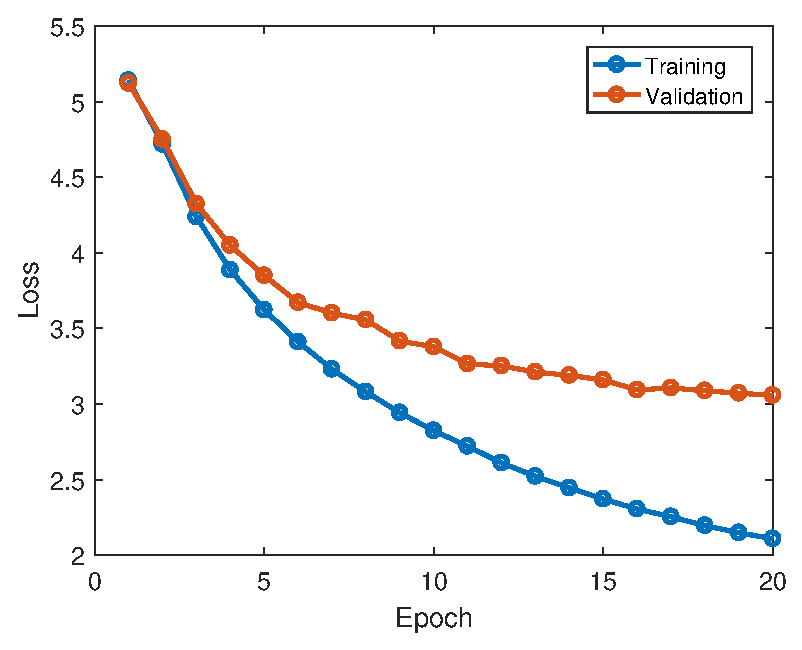
\includegraphics[width=\linewidth]{figs/milestone_loss.eps}
		\caption{Loss history on training and validation sets.}
		\label{fig:loss}
	\end{subfigure}%
	~ %add desired spacing between images, e. g. ~, \quad, \qquad etc.
	%(or a blank line to force the subfigure onto a new line)
	\begin{subfigure}[h!]{0.5\textwidth}
	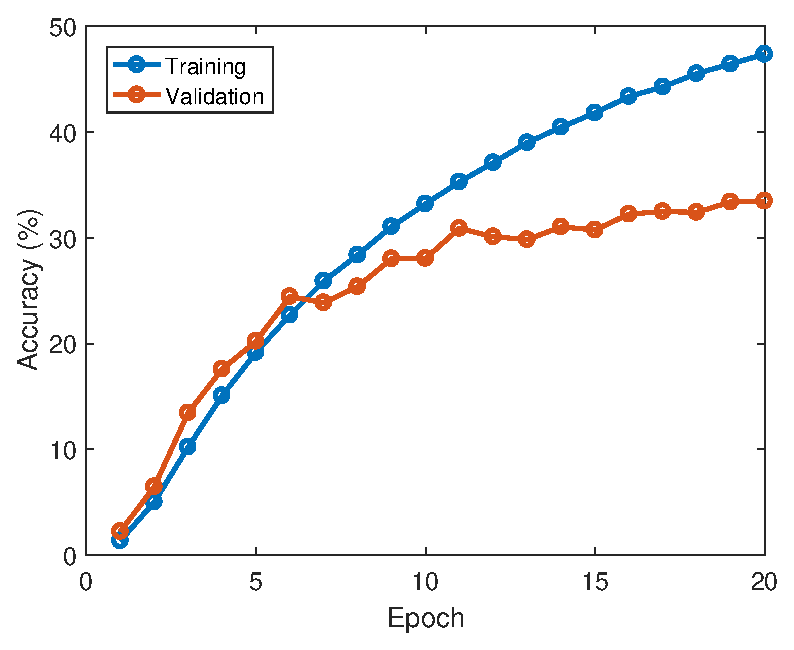
\includegraphics[width=\linewidth]{figs/milestone_accuracy.eps}
	\caption{Classification accuracy on training and validation sets.}
	\label{fig:accu}
	\end{subfigure}
	\caption{Example of (a) loss and (b) accuracy for a VGG16-like network trained from scratch in the Tiny ImageNet data set.}\label{fig:preliminary-results}
\end{figure*}

The fully connected layers of the modified VGG16, VGG19, and ResNet50 networks were trained from scratch. The weights were randomly initialized according to the uniform Glorot initializer \cite{glorot2010}, whereby the weights are uniformly distributed in a range determined by the fan-in and fan-out of the particular layer. The biases were initialized with zeros. 

For all networks, during training of the fully connected layers, the convolutional layers were kept frozen i.e., they were not updated. 

The optimizer for this training stage was Adam with learning rate of $5\times10^{-4}$, $\beta_1 = 0.9, \beta_2 = 0.999, \epsilon=10^{-8}$, and decay = 0.

\subsection{Fine tuning}

Once the fully connected layers had been trained in the transfer learning training stage, there was a subsequent training realized to fine tune the weights of all layers, including the pre-trained convolutional layers.

The motivation for this fine tuning training stems from the fact that the convolutional layers of the networks had been trained on the larger ImageNet challenge with bigger images. Hence, the features extracted in the convolutional layers may not be perfectly suitable for the Tiny ImageNet challenge data set.

The optimizer for this training stage was Adam with learning rate of $1\times10^{-4}$, $\beta_1 = 0.9, \beta_2 = 0.999, \epsilon=10^{-8}$, and decay = 0.

\subsection{Data Augmentation}

To circumvent the problem of the relatively small dataset and to prevent excessive overfitting, I used data augmentation by taking the training images and performing random transformations so that during training, the exact same image is never seen twice. 

To realize data augmentation, I used the \texttt{ImageDataGenerator} class from Keras. This class takes the training data set and performs operations such as rotation, zooming, rescaling, shifts, horizontal flips, and shear transformations. I kept all the control variables to their default values. 

\begin{figure*}[t!]
	\centering
	\begin{subfigure}[h!]{0.5\textwidth}
		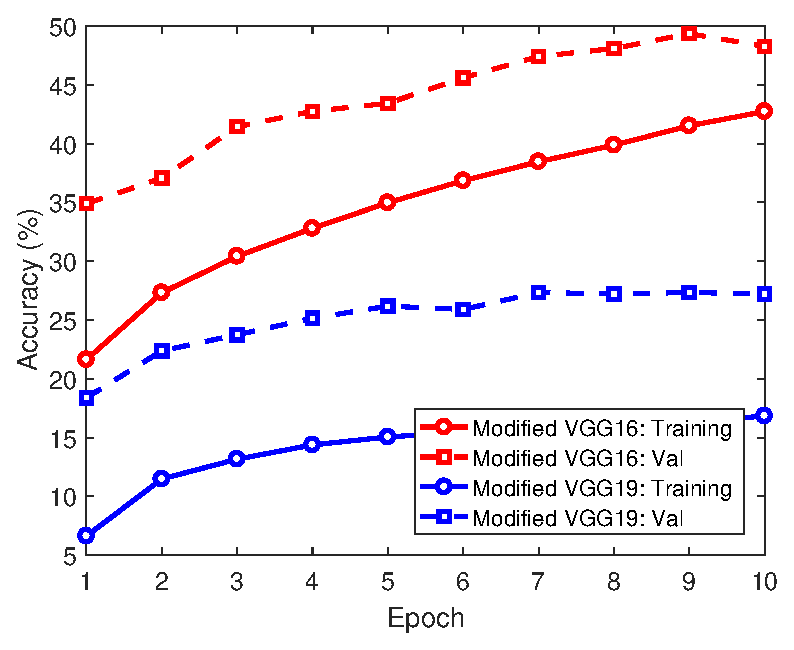
\includegraphics[width=\linewidth]{figs/course_acc_vgg16_vgg19.eps}
		\caption{Accuracy for modified VGG16 and VGG19 during transfer learning training stage i.e., only fully connected layers are trained.}
		\label{fig:course}
	\end{subfigure}%
	~ %add desired spacing between images, e. g. ~, \quad, \qquad etc.
	%(or a blank line to force the subfigure onto a new line)
	\begin{subfigure}[h!]{0.5\textwidth}
		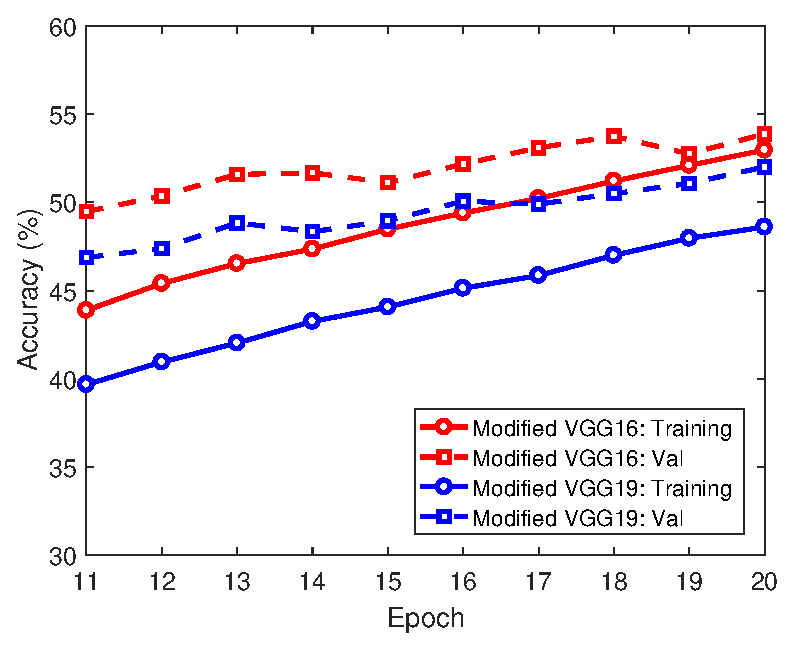
\includegraphics[width=\linewidth]{figs/fine_acc_vgg16_vgg19.eps}
		\caption{Accuracy for modified VGG16 and VGG19 during fine tuning stage i.e., all layers are trained.}
		\label{fig:fine}
	\end{subfigure}
	\caption{Accuracy of modified VGG16 and modified VGG19 during (a) transfer learning, and (b) fine tuning trainng stages.}\label{fig:acc_vgg16_vgg19}
\end{figure*}

\begin{figure*}[t!]
	\centering
	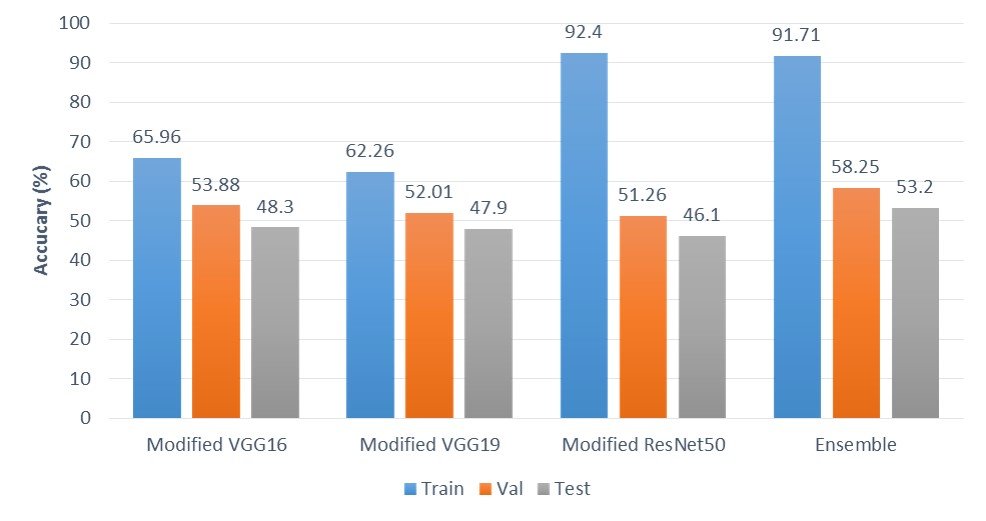
\includegraphics[width=0.99\linewidth]{figs/final_results.jpg}
	\caption{Accuracy of the different network architectures on the training, validation, and testing data sets.}
	\label{fig:final_results}
\end{figure*}

\section{Results} \label{sec:results}

Figure~\ref{fig:acc_vgg16_vgg19}a shows the accuracy evolution for the modified VGG16 and VGG19 networks during the transfer learning stage, where only the fully connected layers are trained. Figure~\ref{fig:acc_vgg16_vgg19}b shows the accuracy evolution during the fine tuning stage, where all the layers are updated. As we can see, despite the modified VGG19 being a deeper network, its performance is virtually the same of that of the modified VGG16 after fine tuning is completed. It appears from Figure~\ref{fig:acc_vgg16_vgg19}b that both networks could achieve even higher accuracy, if trained for longer.

Note that the training accuracy is smaller than the validation accuracy because the training data undergoes random transformations to augment the training data set, while the validation data does not. Without data augmentation in the training set the effects of over fitting become excessively high. 

The performance of all the proposed network architectures, as well as their ensemble are summarized in Fig~\ref{fig:final_results}. 

We see that in the modified VGG16 and modified VGG19 overfitting was successfully mitigated by dropout, $\mathcal{L}2$ regularization, and data augmentation, but this was not the case for the modified ResNet50 network, which exhibited significant overfitting indicated by the gap between training and validation accuracies. 

The modified VGG16 network exhibited performance comparable to the deeper modified VGG19 and modified ResNet50. This highlights the difficulty of training deep networks well. 

The ensemble network, which averages the predicted probabilities of the three other networks, exhibited $\sim5\%$ improved accuracy in the test set, as expected. The ensemble network also exhibits significant overfitting inherited from the modified ResNet50 network. 

\section{Conclusions} \label{sec:conclusion}

I have proposed and trained convolutional neural networks derived from classic network architectures such as VGG16, VGG19, and ResNet50 for the Tiny ImageNet Classification challenge. The networks were trained with transfer learning and subsequently fine tuned with data augmentation. Despite the strategies of dropout, $\mathcal{L}2$ regularization, and data augmentation to mitigate overfitting, there was still noticeable overfitting due to the relatively small data set size. This problem was particularly noticeable in the deeper modified ResNet50 architecture.

The networks achieved high classification accuracy in the test set, with the ensemble network having the highest accuracy of $53.2 \%$ in the test data set. The performance of these  networks could possibly be improved even further by resizing the input images to the same size of the original ImageNet challenge. Moreover, better overfitting management is necessary when training these deep neural networks.

All the code and results in this project are available at \url{https://github.com/jkperin/cs231n/}.

{\small
\bibliographystyle{ieee}
\bibliography{bib}
}

\end{document}
